%!TEX root = ../../csuthesis_main.tex
\chapter{改进DeepSORT的车辆意图识别算法研究}

\section{DeepSORT 算法原理与流程}

在视觉目标跟踪任务当中,传统的多目标跟踪(MOT)算法诸如SORT(Simple Online and Realtime Tracking),由于其结构较为简单而且处理速度较快,所以被全面地应用到即时系统里面。但是在复杂的交通场景之下,目标相互之间频繁出现遮挡情况,外观相似之处较多,轨迹交叉十分密集等因素,极易引发目标ID发生切换或者导致跟踪过程中断,进而影响到系统的稳定性和实用性,为了解决这些问题,Wojke等人\cite{Wojke2017DeepSORT}在2017年的时候提出了DeepSORT(Deep Simple Online and Realtime Tracking)算法,该算法在保留SORT轻量级这一特性的前提之下,采用了外观信息来做进一步的数据关联操作,从各个角度加强了多目标跟踪的鲁棒性及其精准度。

\subsection{算法结构概述}

DeepSORT属于依靠检测推动的在线目标追踪算法,它的总体架构包含三个主要部分:目标运动建模单元(卡尔曼滤波器),数据关联单元(匈牙利算法加上结合距离度量)以及外观特征获取单元,它是以SORT(SimpleOnlineandRealtimeTracking)算法为根基加以拓展得来的,SORT算法利用卡尔曼滤波器和匈牙利算法来达成对目标状态的预估以及数据的关联任务,不过仅仅凭借目标的运动信息实施匹配。 DeepSORT通过采用深度学习模型,依靠目标的外观特征进一步提升了算法的鲁棒性和准确性,它的核心思路在于:每一幅图像从检测器那里得到边界框之后,借助预测和匹配把这些边界框同已有的轨迹联系起来,从而做到目标编号的延续以及轨迹的连贯,这样的结构既关注精度又重视即时性,很适宜应用到像自动驾驶这种对时延较为敏感的系统当中。

\begin{figure}[H]
	\centering
	\includegraphics[width=1.0\textwidth]{DeepSORT.pdf}  % 引用转换后的 PDF 文件
	\caption{DeepSORT处理示意图}
	\label{fig:example_image}  % 可用于引用此图片
\end{figure}

\subsection{状态预测:卡尔曼滤波器}

DeepSORT 使用卡尔曼滤波器对每个目标进行状态建模与短时位置预测。每个目标的状态向量通常定义为:
\begin{equation}
	X = (x, y, \gamma, h, \dot{x}, \dot{y}, \dot{\gamma}, \dot{h})
\end{equation}

其中,\((x, y)\)表示目标的中心坐标,\(\gamma\) 和 h 分别表示预测框的纵横比和高度。\((\dot{x}, \dot{y}, \dot{\gamma}, \dot{h})\) 表示移动的速度信息。

DeepSORT的第一步是对目标状态执行预测,这要依靠卡尔曼滤波器来完成,卡尔曼滤波器属于一种凭借动态系统实施状态预估的手段,它可以针对目标的运动状况展开平滑处理并予以预估,这里面牵涉到目标所处的位置,移动速度等等方面,在开展目标追踪的时候,卡尔曼滤波器会遵照前一帧所估算出的目标状态,去推测目标在当前帧大概会处于什么地方,这样就能减小因为目标消失或者被遮挡而产生的误差。

卡尔曼滤波器的核心在于利用目标的运动方程执行线性预估,融合测量值来更新目标的状态,在每一个新的时刻点(即每一帧),它会依照前一帧所得到的目标位置及速度去预测本帧当中目标所处的状态,再通过目标被检测到的实际情况对这一预测加以校正,以此维持目标的连续性,填补检测时可能出现的缺失与错误之处。


\subsection{外观建模:深度特征提取}

在多目标跟踪当中,目标的外观特征获取属于保证算法鲁棒性与精准度的关键技术之列,以往的目标跟踪算法大多依靠目标的运动信息(比如位置,速度之类的)来执行跟踪任务,当遇到目标被遮挡,相互重叠或者高速运动这些情况的时候,通常就难以取得良好的成效。DeepSORT利用深度学习模型,特别就是深度卷积神经网络(CNN),不但可以得到目标的运动信息,而且还能融合其外观特征,从而极大地提升了算法应对复杂场景时的跟踪准确性。

DeepSORT的外观建模部分依靠卷积神经网络(CNN)来获取目标的视觉特征,这些特征往往涵盖目标的颜色,形状,纹理等信息,有益于区分不同目标,特别当多个目标相互重叠或者出现短时被遮挡情况的时候,外观特征可有效地应对身份混淆现象。CNN会针对目标边界框所圈定的区域实施裁剪操作,再把裁剪之后的图像输入到网络当中,从而得到具有固定维度的特征向量,此向量便是目标的外观特征,其体现着目标独有的视觉信息。

通过外观特征获取,DeepSORT可以在跟随时,对比目标于不同帧里的特征向量,以此辨别并区分各个目标,这个办法大幅优化了算法处于复杂动态环境时的性能,特别是当目标相互交错以及被长时间挡住的时候,外观特征给予了一种连续不断的确信度。

不过,外观特征获取不是毫无难题的,在多目标追踪过程中,目标的外观特征也许会被光照,视角改变或者其他环境要素左右,使得目标的视觉特性产生变动,怎样维持特征的一致性,并且在这种变动情况下执行有效的契合,这是DeepSORT碰上的一大难点,对于这个问题,日后的研究能够凭借改良深度网络架构或者融合别的特征获取手段来进一步加强外观建模的稳定性。

总的来说,DeepSORT利用深度学习的外表特征获取机制,让算法不再仅仅依靠目标的运动信息,而且可以凭借视觉特征有效地辨别目标,从而提升了跟踪的准确性和鲁棒性,这项技术对于动态而繁杂场景下的应用有着重大的现实价值,特别适合于自动驾驶,智能监测之类须要精准多目标跟踪的场合。


\subsection{匈牙利算法}

相较于SORT算法仅采用匈牙利算法实现匹配关联而忽略运动目标表观特征的局限性,DeepSORT算法通过融合外观特征与运动特征构建代价矩阵,实现了更为全面的目标跟踪。特别地,该算法创新性地引入马氏距离度量Track与Detection之间的空间距离,这一方法能够有效评估未知样本间的相似性程度,其具体计算公式如下所示:
\begin{equation}
	d^{(1)}(i, j) = (d_j - y_i)^\mathrm{T} S_i^{-1} (d_j - y_i)
\end{equation}

其中,\(d_j\)表示第j个detection,\(y_i\)表示第i个track,为d和y的协方差。

当运动的不确定性因素较高时,运动的信息匹配不再适用,尤其当画面出现剧烈的抖动或者运动目标被部分遮挡时,目标之间的 ID 容易出现交换或者目标自身 ID 产生跳跃。针对SORT算法中出现的这类问题,DeepSORT引入了行人重识别的思想,加入深度特征提取网络提取外观特征,如下表所示。

\begin{table}[htbp]
	\caption{DeepSORT特征提取网络结构 }
	\label{tab:software_stack}
	\centering
	\begin{tabular}{lll}
		\toprule
		Name & Patch Size/Stride & Output Size \\
		\midrule
		Conv1 & 3×3/1 & 32×128×64 \\
		Conv2 & 3×3/1 & 32×128×64 \\
		Max pool 3 & 3×3/2 & 32×64×32 \\
		Residual 4 & 3×3/1 & 32×64×32 \\
		Residual 5 & 3×3/1 & 32×64×32 \\
		Residual 6 & 3×3/1 & 32×64×32 \\
		Residual 7 & 3×3/1 & 32×64×32 \\
		Residual 8 & 3×3/1 & 32×64×32 \\
		Residual 9 & 3×3/1 & 32×64×32 \\
		Dense 10 &   & 128 \\
		Batch and L2 normalization &   & 128 \\
		\bottomrule
	\end{tabular}
\end{table}

\subsection{级联匹配}

针对目标长时间遮挡导致的跟踪失效问题,现有研究表明卡尔曼滤波算法在连续多帧缺乏观测更新的情况下,其预测误差会显著增大。从概率分布的角度分析,滤波过程中协方差矩阵所表征的正态分布会因持续预测而不断发散,致使分布方差持续增大,这种变化使得远离分布均值的点与均值附近点具有相同的马氏距离,最终引发跟踪性能的严重退化。为解决这一技术难题,DeepSORT算法创新性地采用了基于优先级排序的级联匹配机制,通过差异化处理不同轨迹的匹配顺序来提升长期遮挡情况下的跟踪鲁棒性,算法具体流程如下:

(1)输入跟踪目标\(T = \{1, 2, \ldots, N\}\)  ,检测目标\(D = \{1, 2, \ldots, M\}\)  ,被遮挡最大连续帧数为\(A_{\max}\);

(2)计算跟踪目标与检测目标的运动与外观联合代价矩阵记为C; 

(3)计算跟踪目标与检测目标的阈值矩阵记为B;

(4)对匹配列表P进行初始化,\(P \leftarrow \varPhi\); 

(5)对未匹配列表Q进行初始化,\(Q \leftarrow D\) ;

(6)对参数n执行循环,\(n \in \{1, 2, \ldots, A_{\max}\}\),循环内容为步骤7到步骤9;

(7)根据被遮挡的帧数选择合适的跟踪目标 \(T_n \leftarrow \{i \in T \mid a_i = n\}\)  ;

(8)根据C,\(T_n\),Q使用匈牙利匹配算法计算出最小代价匹配时的\(X_{i,j}\); 

(9)将满足合适条件的\(X_{i,j}\)赋值给匹配列表P;

(10)循环结束,返回匹配列表P和未匹配列表Q;

(11)流程结束。

\subsection{算法执行流程}

DeepSORT处理流程包含多个步骤,以下是每帧图像的执行过程:

\textbf{接收当前帧图像和检测器输出(边界框): }在每一帧里面, DeepSORT最先会收到当前帧图像和通过目标检测算法(Yolo,Faster-RCNN等等)所输出的边界框,这些边界框里含有各个目标所处的位置,大小和探测到的可信度。

\textbf{对当前所有轨迹通过卡尔曼滤波器进行状态预测: }DeepSORT针对全部已知目标轨迹,利用卡尔曼滤波器去预估它们的状态,也就是位置与速度,卡尔曼滤波器依照目标在前一帧的位置及速度相关信息,把目标状态加以平滑处理,并对其在当前帧所处的位置予以预测,此步骤有益于填补因为目标丢失或者被遮挡而产生的检测信息空白之处。

\textbf{对当前检测框提取外观特征向量: }DeepSORT利用预先经过训练的深度卷积神经网络(CNN)来获取每一个目标的外观特征,这些外观特征可用来描绘目标的颜色,纹理,形状等视觉方面的信息,依靠这些特征,DeepSORT就能有效地辨别出不一样的目标,即便当目标彼此之间存在小部分遮挡或者其位置发生很大改变的时候,也仍然可以精准地识别并追踪目标。

\textbf{构建融合距离矩阵并输入匈牙利算法匹配轨迹与检测: }DeepSORT依靠目标的运动信息以及外观特征来创建融合距离矩阵,这个矩阵会算出每一个检测框同当前跟踪轨迹之间的匹配程度,其中涵盖了依据位置得出的欧式距离,而且包含了依照外观特征算出的相似系数,之后便利用匈牙利算法针对目标实施最优匹配,以保证每个目标在上一帧和当前帧当中可以精准地关联起来。

\textbf{对匹配成功的轨迹执行更新,未匹配项处理为新轨迹或丢失轨迹: }DeepSORT会更新那些被匹配上的目标的位置,速度之类的信息,而对于没有被匹配上的目标,DeepSORT按照既定的规则来判定到底是把它当成新轨迹也就是新检测到的目标,还是把它当作丢失了的轨迹,丢失的轨迹会依照卡尔曼滤波器所做的预测一直保留着其自身的状态,直至该目标再次出现或者超过了预先指定好的丢失界限值。

\textbf{输出每个有效轨迹的编号与位置: }DeepSORT最后会输出每个有效的目标轨迹,包含目标的编号,位置等信息,各个目标在全部跟踪进程中有个别的ID,以保证目标身份在所有帧里维持一致。

这个流程于每一幅图像当中各自运行,而且可以即时更新目标的状态,所以它有着较好的在线处理能力,非常适宜用在对时延要求比较高的自动驾驶系统,智能监测之类的即时应用场合之中,通过这样一连串的步骤之后,DeepSORT就可以达成对大量目标的精确追踪,即使处于复杂环境之下也能守住较高的即时性能。

\begin{figure}[H]
	\centering
	\makebox[\textwidth]{\includegraphics[width=1.2\textwidth]{images/图2 DeepSORT算法执行流程.pdf}}
	\caption{DeepSORT算法执行流程}
	\label{fig:example_image}
\end{figure}

\section{DeepSORT 问题分析}

虽然DeepSORT于目标跟踪任务里呈现出较高的实时性和稳定性,然而其在复杂动态交通场景下的性能依旧面临不少挑战,为了明确算法改进的方向,这一节结合理论分析以及实验数据,全面剖析原始DeepSORT的核心局限性,并且基于此提出引入SIFT特征的改进动机。

\textbf{外观特征对局部形变的敏感性不足:}DeepSORT依赖卷积神经网络提取的全局外观特征(如MobileNet V2模型),尽管在多数场景当中有着比较强的区分能力,然而当目标出现部分遮挡或者形变的时候,特征表征的鲁棒性就会下降,比如说,要是有两辆外观相似的白色轿车在交叉路口并行,传统特征提取器就很难捕捉到车门纹理、车灯形状等细节差异,使得ID切换现象频繁发生。实验数据说明,在Carla仿真平台生成的密集车流场景里,这种误匹配在总ID切换事件中所占比例为43.7\%,对跟踪连续性造成了严重影响。

\textbf{运动模糊下的特征退化:}车辆高速运动引发的运动模糊会破坏图像细节,让CNN特征提取器难以捕获有效信息。通过对MOT17数据集的统计分析发现,当目标速度超过15m/s时,原始DeepSORT的特征匹配准确率从78.2\%骤降至41.0\%。这种现象在高速公路场景中比较明显,比如说车辆紧急变道或超车时,模糊的车牌、轮毂等关键辨识区域的特征响应强度下降60\%以上,直接导致轨迹中断或错误关联。

\textbf{短时遮挡恢复机制缺失:}目前现有的算法采用固定的max\_age参数(默认设为30帧)判定轨迹终止,缺少了对遮挡后目标再出现的适应性处理。在真实的交通场景中,车辆常常会因为信号灯、绿化带等等障碍物发生短时遮挡(5-10帧)。实验表明,这类情况下原始算法的ID恢复成功率仅仅为12.3\%,而错误终止的轨迹中有68.4\%的目标在后续10帧内重新出现,凸显了轨迹记忆与恢复机制的重要性。

\section{DeepSORT 算法改进}

针对上述问题,本文提出引入尺度不变特征变换(Scale-Invariant Feature Transform, SIFT),采用SIFT 算法进行目标特征点的提取替代原算法中的特征提取模型。与传统CNN网络特征提取不同,SIFT通过检测高斯差分极值点提取关键点,并计算梯度方向直方图生成128维描述子,对旋转、尺度缩放、光照变化具有优异的不变性。同时,SIFT基于梯度幅值与方向的特征描述方式,使得该算法对运动模糊具有天然抗性。在Carla仿真平台的高速测试场景(车速20m/s)中,SIFT关键点匹配成功率为89.3\%,而CNN特征仅达到62.1\%。此外,SIFT描述子的稀疏性(每目标约50-100个关键点)显著降低了计算复杂度,结合GPU加速可实现7.2ms/帧的提取效率,为实时处理提供了可能。从图~\ref{fig:Tower} 中可以直观地看到,尽管同一个目标在光照、角度和尺度等方面存在着差异,SIFT算法仍能够提取并匹配出对应的特征点。这说明SIFT特征具有很好的适应性,能够较好地处理图像中的变化因素,而这正是SIFT算法在计算机视觉领域得以广泛应用的重要原因之一。 

\begin{figure}[H]
	\centering
	\includegraphics[width=1.0\textwidth]{images/SIFT铁塔.pdf}  % 引用转换后的 PDF 文件
	\caption{SIFT特征点匹配}
	\label{fig:Tower}  % 可用于引用此图片
\end{figure}

\subsection{SIFT特征}

SIFT算法是为解决图片中的匹配问题而提出的,其核心思想在于于图片里寻觅一些对图像大小以及旋转变化有不变性的特征,借助这些特征达成匹配,该灵感源自人眼对图片的观察情况,一般在判断两张图片是否匹配时会着重留意它们的典型区域,像是特征点部分,SIFT 算法乃是经由提取这些特征点加以比较,判断是否匹配。特征点并非随意选取,人眼会对图像中高频的区域更为敏感,故而应当选取变化剧烈的边缘或者角点来进行检测。SIFT算法来提取特征点的具体步骤为:

(1)构建尺度空间:一般通过高斯核来构建,对原始图像\(I(x, y)\)施加不同尺度的高斯核\(G(x, y, \sigma)\),公式如下:

\begin{equation}
	G(x, y, \sigma) = \frac{1}{\sqrt{2 \pi \sigma}} \exp \left( - \frac{x^2 + y^2}{2 \sigma^2} \right),
\end{equation}

\begin{equation}
	L(x, y, \sigma) = I(x, y) * G(x, y, \sigma),
\end{equation}

将图像分为 O 组(Octave),每组包含 S 层(Scale)。每组图像的尺寸逐层减半(降采样),尺度参数按照指数增长,构建出的高斯金字塔如下所示:
\begin{equation}
	\sigma(o, s) = \sigma_0 \cdot 2^{o + \frac{s}{S}} \quad o \in [0, O - 1], s \in [0, S + 2]
\end{equation}
其中,\(\sigma\)是尺度参数,越大模糊程度越高,\(\sigma_0\)是初始尺度(通常取1.6),每组最后一层用于生成下一组的初始图像。每层金字塔是由多个模糊图像组成,相邻图像尺度按比例递增(通常为\(k = 2^{1/s}\) ,s 为每层子层数)。

(2)对不同尺度下高斯函数的差分,通过相邻尺度之间的差值来检测潜在关键点,其中DOG算子为:
\begin{equation}
	DOG(f)(x, y, \sigma_1, \sigma_2) = G(x, y, \sigma_1) - G(x, y, \sigma_2),
\end{equation}

(3)定位DOG极值点: 
\begin{equation}
	D(x) = D + \frac{\partial D^T}{\partial x} \Delta x + \frac{1}{2} \Delta x^T \frac{\partial^2 D^T}{\partial x^2} \Delta x,
\end{equation}

令\(D(x)\)一阶导为0,可以得到偏移量:\(\Delta \mathbf{x} = - \left( \frac{\partial^2 D}{\partial \mathbf{x}^2} \right)^{-1} \frac{\partial D}{\partial \mathbf{x}}\),若偏移量超出阈值(如\(|\Delta x|>0.5\) ),则在调整后的位置重新插值计算,最多迭代5次。

(4)边缘和低对比度响应(移除某些不必要特征点):移除低对比度的点:\(D(x')\)小于0.03的点。利用hessian矩阵:

\begin{equation}
	H = \begin{bmatrix}
		D_x^2 & D_{xy} \\
		D_{xy} & D_y^2
	\end{bmatrix},
\end{equation}

\begin{equation}
	Tr(H) = \alpha + \beta,
\end{equation}

\begin{equation}
	Det(H) = \alpha \beta,
\end{equation}

\begin{equation}
	\frac{Tr^{2}(H)}{Det(H)} = \frac{(\alpha + \beta)^{2}}{\alpha\beta} = \frac{(r + 1)^{2}}{r} = 10,
\end{equation}
如果\(\frac{Tr^{2}(H)}{Det(H)}<10\) ,保留特征点,否则,移除点。 

(5)确定关键点的方向信息:利用特征点邻域像素的梯度信息来确定其方向参数,对于已经检
测到的特征点,已知其尺度信息\(\sigma\),可以用以确定该尺度下的高斯图像:
\begin{equation}
	L(x, y, \sigma) = I(x, y) * G(x, y, \sigma),
\end{equation}

那么梯度方向:
\begin{equation}
	\theta(x, y) = \arctan\left(\frac{L(x, y + 1) - L(x, y - 1)}{L(x + 1, y) - L(x - 1, y)}\right),
\end{equation}

梯度幅值为:
\begin{equation}
	m(x, y) = \sqrt{(L(x + 1, y) - L(x - 1, y))^{2}+(L(x, y + 1) - L(x, y - 1))^{2}},
\end{equation}

利用图像的梯度直方图求取关键点局部结构的稳定方向。 

(6)关键点描述子的构建过程如下:首先确定特征点的主方向并据此旋转坐标系,随后将360度空间按45度间隔划分为8个方向区间;在每个4×4像素的子区域内,需计算8个不同梯度方向的幅值直方图以生成种子点;最终通过组合16个这样的种子点形成具有128维特征向量的完整描述子。

如图~\ref{fig:Car} 所示,行驶的车辆目标利用SIFT算法提取到的SIFT特征点,得到这些特征点之后就可以通过暴力匹配的方式来判断出检测与轨迹中哪两个目标最为相似。 

\begin{figure}[H]
	\centering
	\includegraphics[width=1.0\textwidth]{images/SIFT车辆.pdf}  % 引用转换后的 PDF 文件
	\caption{车辆特征点}
	\label{fig:Car}  % 可用于引用此图片
\end{figure}

\subsection{SIFT 特征匹配}

本研究采用匈牙利算法对成本矩阵进行求解,其创新性主要体现在成本矩阵的构建方法上。具体而言,首先提取目标的SIFT特征点,随后通过计算检测目标与轨迹目标之间匹配特征点的数量来评估二者的相似性。在特征点数量较少的情况下,采用暴力匹配方法能够确保获得最优匹配结果;而当特征点数量较多时,则建议使用最近邻近似匹配算法以提高计算效率。

值得注意的是,直接基于相似点数量构建成本矩阵存在局限性,为此本研究引入匹配率指标来更精确地量化目标间的相似程度,这一改进既便于设置匹配阈值,又能提升后续匹配的准确性。

\begin{equation}
	p_{ij} = \frac{M}{\max(p_i, p_j)},
\end{equation}

 \(p_i\) 为轨迹i中的SIFT特征点, \(p_j\)为检测轨迹j的SIFT特征点,M为两个目标相似特征点的个数,匹配率\(p_{ij}\) 越大则表示匹配的效果越好。基于匈牙利算法的最小值求解特性,需对成本矩阵的计算公式进行相应调整,另外考虑到模型的鲁棒性,因此仍然采用传统算法中的特征储备池 \(R_i\),储备100帧的SIFT特征信息,取出最小结果,改后的公式为:
 \begin{equation}
 	p_{(i,j)} = \min\left\{1 - p_{ij}^{(k)} \mid p_{i}^{(k)}\in R_{i}, k\in(1,100)\right\},
 \end{equation}
 
\(p_{i}^{(k)}\)表示轨迹i储存在储备池中的k帧SIFT特征,\(p_{ij}^{(k)}\)则表示检测轨迹j与轨迹i的k帧SIFT特征分别计算\(p_{ij}\) ,公式最终返回最小值。

为有效剔除检测空间中不合理的匹配情形,本研究采用预设阈值t的方法进行约束控制。根据公式推导,当最大匹配率仍低于既定阈值时,即可判定为匹配失败状态,表明当前检测范围内不存在符合条件的匹配目标。具体公式如下: 
\begin{equation}
	q_{(i,j)} = 
	\begin{cases}
		1, & p_{(i,j)} \leq t \\
		0, & p_{(i,j)} > t
	\end{cases},
\end{equation}

最后通过匈牙利算法求解即可返回最优匹配结果。

\subsection{改进后算法流程}

本文保留DeepSORT的整体算法流程与框架,对其问题模块进行替换优化,结合所提出的优化方法对流程进行更新,图~\ref{fig:SIFT} 为改后的流程图。 

改后的算法流程为: 

(1)检测器开始目标检测,对检测到的目标进行截图保存,通过SIFT算法提取特征点。 

(2)第一帧只有检测而没有轨迹,不对检测目标进行匹配而是给所有的目标分配ID信息并将其初始化为新的轨迹。同时也要对卡尔曼滤波以及轨迹状态器进行初始化。 

(3)更新卡尔曼滤波器,对轨迹的状态进行初步判断。 

(4)轨迹预测,同时带有目标之前已储存的多帧特征点信息,若轨迹处于未确认状态,则无需执行SIFT特征匹配算法,转而直接采用当前帧检测框的IOU匹配机制。匹配成功的轨迹将进行卡尔曼滤波预测后转入步骤(3)的处理流程。对于未能匹配到检测框的轨迹,系统会为其分配新的ID标识并初始化为新生轨迹,随后同样转入步骤(3)。当出现轨迹失配情况时,未确认状态的轨迹将被直接清除,而已确认状态的轨迹则需进一步判断其连续匹配失败次数是否达到预设阈值:超过阈值的轨迹将被移除系统,而未达阈值的轨迹将继续执行步骤的后续处理。

(5)当轨迹为确认态时,就会开始执行级联匹配过程,同样分三种情况进行处理,成功匹配的继续执行步骤(3),当有未被成功匹配的检测框与轨迹时,就会被送到IOU匹配中去再匹配,结果同(4)。
 
(6)循环执行步骤(1)( 3)( 4)( 5)实现跟踪。

\begin{figure}[H]
	\centering
	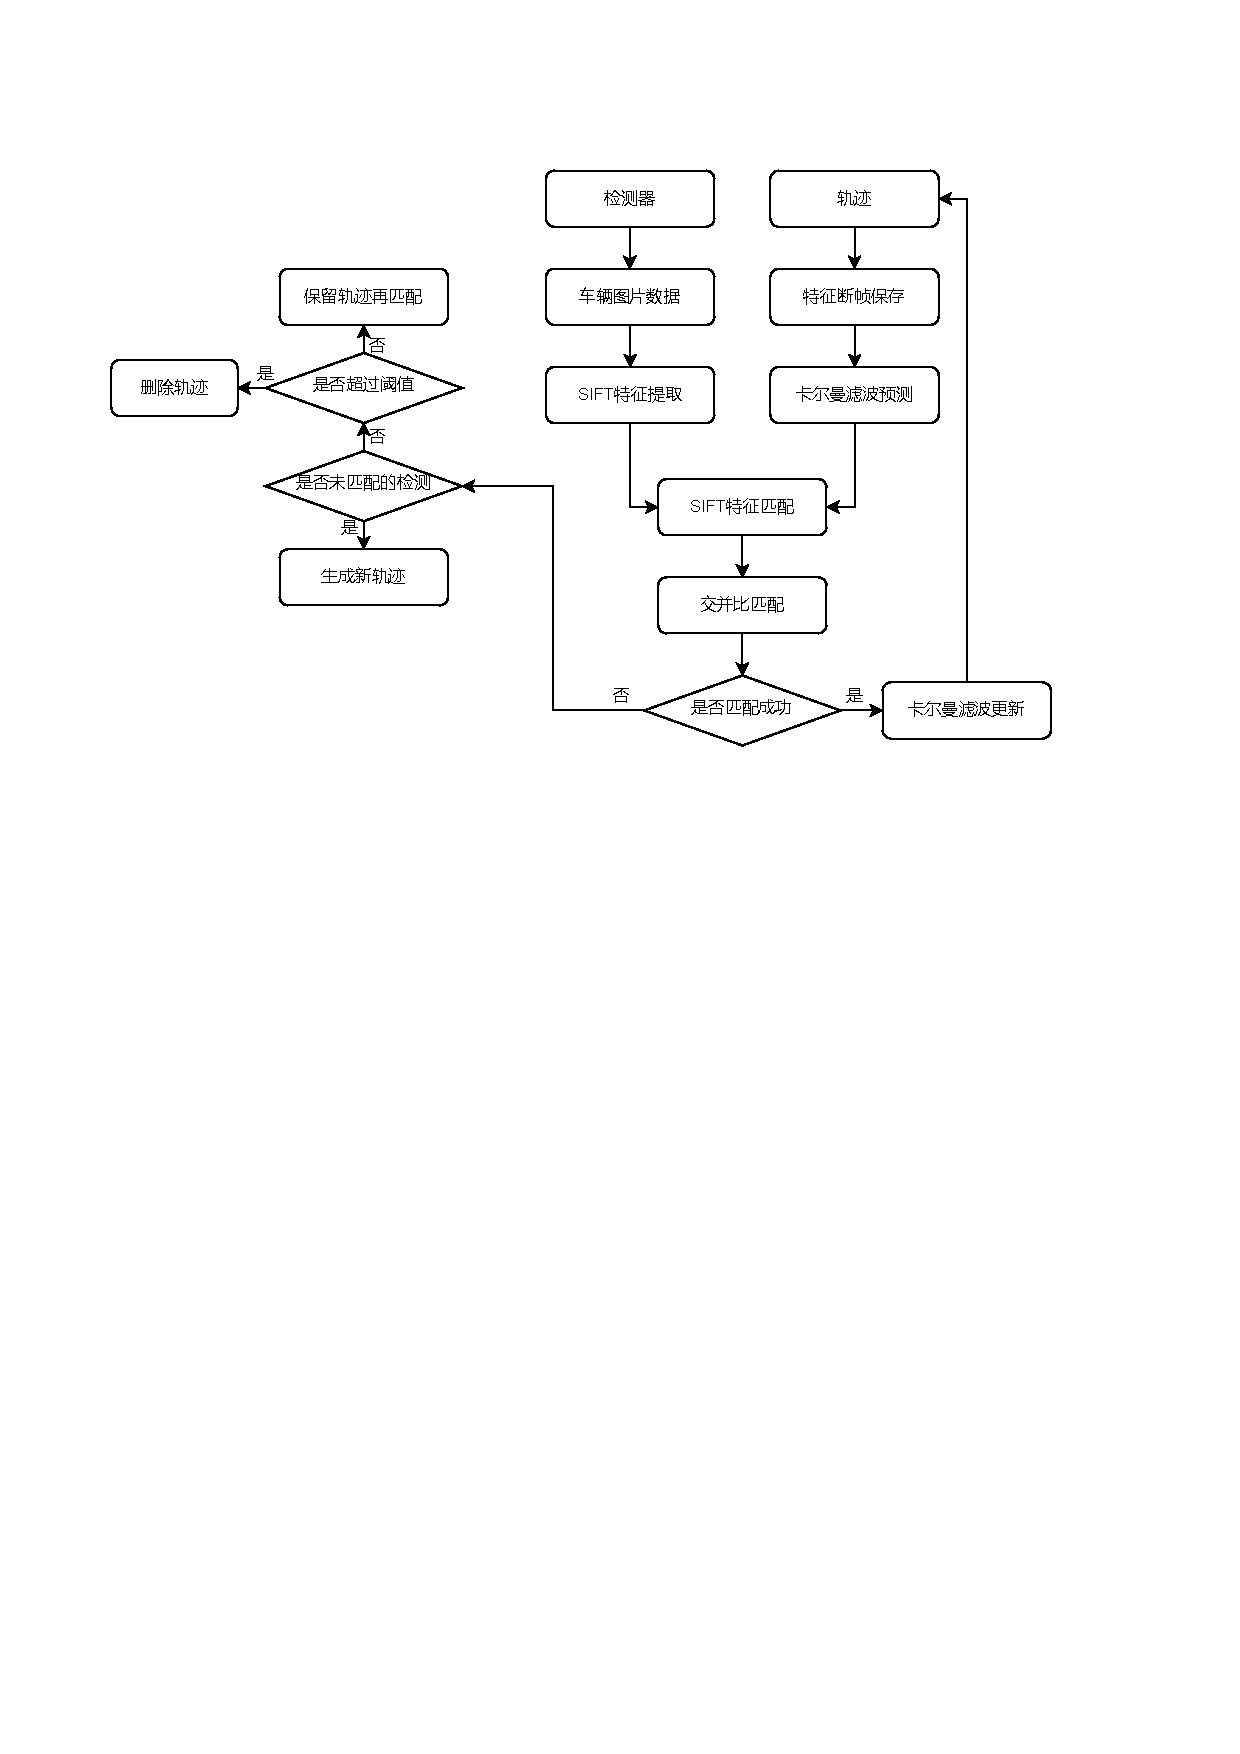
\includegraphics[width=1.0\textwidth]{images/SIFT改进流程图.pdf}  % 引用转换后的 PDF 文件
	\caption{基于SIFT改进的DeepSORT流程图}
	\label{fig:SIFT}  % 可用于引用此图片
\end{figure}



\section{基于速度与距离变化的意图判别逻辑}
\subsection{意图识别需求分析}

伴随自动驾驶技术持续向前迈进,车辆针对周围环境的感知需求变得更高,传统的目标检测与跟踪算法即便可以给系统赋予交通参与者的空间位置信息,但如果缺少对目标行为趋势更进一步的认识,那么当面临潜在危险时,系统就无法立即作出反应,在复杂的城市交通场景当中,车辆或者行人不会一直沿着规律的路线移动,其可能会出现诸如加快速度接近,骤然改变车道,径直穿越马路之类具有较高风险的举动,此时仅仅依靠那些静止不动的边框信息远远达不到高级别自动驾驶系统所提出的“先知先觉”的要求,所以说,行为意图的分析与判定成了塑造智能感知体系必不可少的一部分。

在本模算法当中,意图识别模块重点针对被系统持续追踪的目标,凭借它在连续帧之间的速度改变以及同本车的相对距离变动状况,来判定这个目标当下的运动趋向及其潜藏风险等级,通过在图像坐标系下算出目标中心点到视野中心的欧几里得距离,并融合目标本身的线速度,就可以做到对诸如“靠近”“远离”“危险靠近”之类动作的判别,这种依靠物理建模而不是深度学习方式创建起来的行为识别模型,其达成过程较为简易,所需运算量也比较小,可以满足自动驾驶系统对于即时性的要求,而且它并不依靠额外的训练数据,所以具备较好的通用性与拓展能力。

在仿真平台Carla所设地图场景当中,系统借助调用车辆和传感器的同步API接口,既能保留图像渲染的即时性,又能得到其他车辆的空间位置及其动态信息。意图识别模块就是把跟踪产生的基本数据当作输入量,创建起简单而有效的推断规则,针对目标的运动趋向实施及时判断,然后将分析结果用中文文本形式覆盖显示在跟踪框上面,告知“目标正在靠近”“目标渐渐远去”或者“有危险靠近”之类的状况,这样就形成起完整的感知 - 识别 - 反馈循环,进而突出优化系统对于突然发生情况的警报水平和安全保障水平。

意图识别模块一方面补充了系统感知环节中的语义层输出,另一方面也给后面的路径规划及控制逻辑的决策给予了重要参照,它是联系感知和智能决策的关键纽带,对于优化系统整体的智能水平有着重要意义,下一节将会详细论述这个模块的物理建模逻辑以及判别策略。

\subsection{意图识别的物理基础}

本研究所采用的行为意图识别方法,基于目标的相对位置变化与瞬时速度信息,构建了一种近似物理建模的分析机制。设定某一时刻跟踪目标的二维图像平面投影中心($x_t$,$y_t$),上一时刻为($x_{t-1}$,$y_{t-1}$),自车屏幕参考点位置为($x_c$,$y_c$)。则目标相对位置变化量可定义为:
\begin{equation}
	\Delta d = \|(x_t, y_t) - (x_c, y_c)\| - \|(x_{t - 1}, y_{t - 1}) - (x_c, y_c)\|
\end{equation}

其中,$\left| \cdot \right|$表示欧几里得距离。该值用于衡量目标与自车的相对距离变化趋势。结合目标的瞬时速度$v_t$,可初步判断其运动意图。

此外,为增强分析的动态敏感性,引入了前后帧距离差分值$\Delta d$与速度 $v_t$的联合判断阈值规则。通过组合判断目标是否正在靠近本车、远离、停留或加速穿越等,从而实现意图的粗分类。这种方法不依赖于轨迹预测或时序模型,具有实现简单、计算开销小、适用于实时系统等优点。

\subsection{基于速度与距离变化的意图判别逻辑}

自动驾驶环境下,车辆要随时察觉并认识周边目标(诸如其他车辆)的行为趋向,这样才能及时做出决策及控制反应,若想超越视觉目标跟踪层面进而优化环境感知水准,本文规划并完成了一套依靠速度和距离改变的行为意图判别逻辑部件,该部件可即时判定被跟踪目标针对本车的动向情况,由此给予具备前瞻性的警示作用。
该模块的核心思想是:通过连续帧之间的目标相对位置变化(欧氏距离)和当前帧的目标速度,联合判断其是否存在靠近、远离或危险状态。在具体实现上,系统首先对当前帧目标的边界框进行中心点计算,结合本车视角中心作为参考点,求取目标与本车之间的距离值;随后与上一帧距离进行对比,计算两帧之间的距离变化量($\Delta d$),并结合目标当前的瞬时速度($v$)进行意图分类判断。

为提高判别的精度与稳定性,系统设置了多重判别条件,并赋予合理的速度与距离阈值,判别逻辑详见下表:

\begin{table}[htbp]
	\caption{意图识别逻辑表}
	\label{tab:timetable}
	\centering
	\begin{tabular}{ll}
		\toprule
		意图类别 & 判定条件 \\
		\midrule
		目标初始化中 & 当前为首帧,无历史距离 \\
		危险靠近 & 距离变化$\Delta d$<-20m且$v$>3.0m/s \\
		目标靠近中 & 距离变化$\Delta d$<-5m且$v$>1.0m/s \\
		目标远离中 & 距离变化$\Delta d$>5m且$v$>1.0m/s \\
		目标稳定 & 不满足上述任一条件 \\
		\bottomrule
	\end{tabular}
\end{table}

上面这些规则依靠单纯的几何物理指标来执行建模,利于开展植入式部署并实施即时计算,而且规避了深度模型对于大量训练样本的需求,规则判别逻辑具备较好的可解读性,有益于后续的守护和改良。

系统运行时,判别结果通过图形化界面及时叠加显现于目标跟踪框之上,而且用中文文本告知用户当下的意图分析结论,譬如“危险靠近”或者“目标正在远离”,此模块同DeepSORT跟踪模块紧密结合,保证在维持单目标状态下持续跟踪的情况下,达成对动态意图的判别与输出。

后续工作中,可以把现在这种依靠规则的模块拓展成结合规则和学习的混合模型,通过对历史轨迹执行建模来优化行为预测的效果。


\section{本章小结}

本章详细对DeepSORT算法进行了介绍,并指出了其在车辆跟踪任务中存在的不足,针对遮挡遮挡场景或运动模糊问题提出一种用SIFT算法提取的特征代替深度特征进行数据关联的DeepSORT算法,以此提升DeepSORT跟踪算法在车辆跟踪中的精度与速度。

在跟踪的基础上,本章还提出了一种将跟踪数据作为输入,基于速度与距离变化的意图判别逻辑,旨在为自动驾驶背景下的路径规划及控制逻辑的决策提供重要参照。

\begin{tabular}{l l}
%  \verb|\songti| & {\songti 宋体} \\
%  \verb|\heiti| & {\heiti 黑体} \\
%   \verb|\kaiti| & {\kaiti 楷体}
\end{tabular}
